\documentclass[a4paper,12pt]{article}

\usepackage{setspace}
\usepackage{xcolor}
\usepackage{graphicx}
\usepackage{geometry}
\usepackage{float}
\usepackage{titlesec}
\usepackage{subfigure}
\usepackage{caption}
\captionsetup{figurewithin=section}
\usepackage{amsmath}
\usepackage{listings}
\usepackage{xcolor}

\begin{document}

\title{\textbf{Homework 3}}
\author{Yunian Pan}
\maketitle{}


\section{Optimization}

I did normalization on the loss function to avoid numerical problem:
\begin{equation}
   J = -\frac{1}{N}\sum_{i=1}^{N} \log(\sigma(y_i w_i^{\top} k_i)) + \lambda w^{\top} w \nonumber 
\end{equation}

The gradient then becomes:

\begin{equation}
    \nabla_{w}J = -\frac{1}{N}column[(1- \sigma(y_i w_i^{\top} k_i)) y_i k_i^{\top}] + 2  \lambda  w \nonumber 
 \end{equation}


\subsection{GD}

After some exploration, I set the parameters are as below and get the results:

\begin{table}[htbp]
    \caption{GD}
    \label{GD-table}
    \centering
    \begin{tabular}{lll}
      $\lambda$     &  1e-3 \\
      $step\ size$ &   2e-3   \\
      $\epsilon$     &  1e-5     \\
      step length     &   3000 \\
      accuracy & 90.2\% 
    \end{tabular}
  \end{table}

The learning curve is in $\ref{GD}$
  \begin{figure}[htbp]
    \centering
    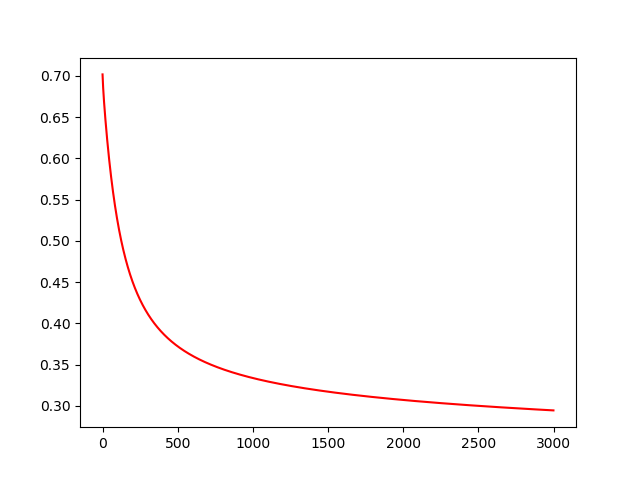
\includegraphics[width = .8\textwidth]{GD}
    \caption{GD}
    \label{GD}
\end{figure}


\subsection{SGD}

For SGD, first I tried the window size $p = 1$

\begin{table}[htbp]
    \caption{SGD1}
    \label{SGD1-table}
    \centering
    \begin{tabular}{lll}
        p & 1 \\
      $\lambda$     &  1e-3 \\
      $step\ size$ &   3e-4   \\
      $\epsilon$     &  1e-5     \\
      step length     &   3000 \\
      accuracy & 88.9\% 
    \end{tabular}
  \end{table}

The learning curve is in $\ref{SGD1}$
  \begin{figure}[htbp]
    \centering
    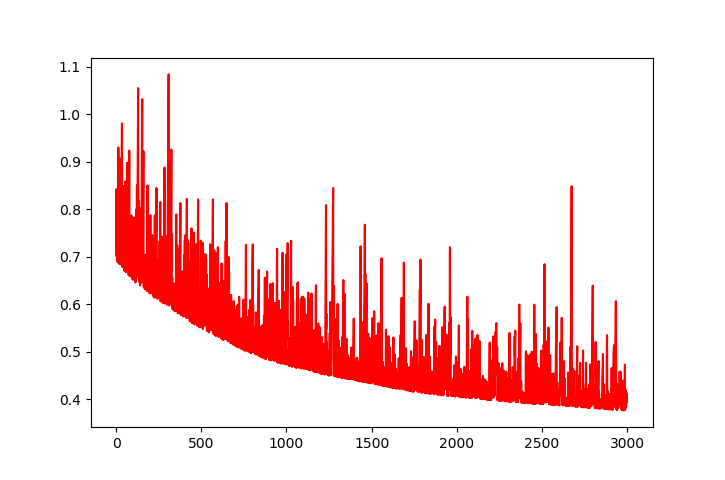
\includegraphics[width = .8\textwidth]{SGD1}
    \caption{p = 1}
    \label{SGD1}
\end{figure}


For the setting of $p = 100$, as $\ref{SGD100-table}$ shows,

\begin{table}[htbp]
    \caption{SGD2}
    \label{SGD100-table}
    \centering
    \begin{tabular}{lll}
        p & 100 \\
      $\lambda$     &  1e-3 \\
      $step\ size$ &   3e-4   \\
      $\epsilon$     &  1e-5     \\
      step length     &   3000 \\
      accuracy & 91.2\% 
    \end{tabular}
  \end{table}

The learning curve is in $\ref{SGD100}$
  \begin{figure}[htbp]
    \centering
    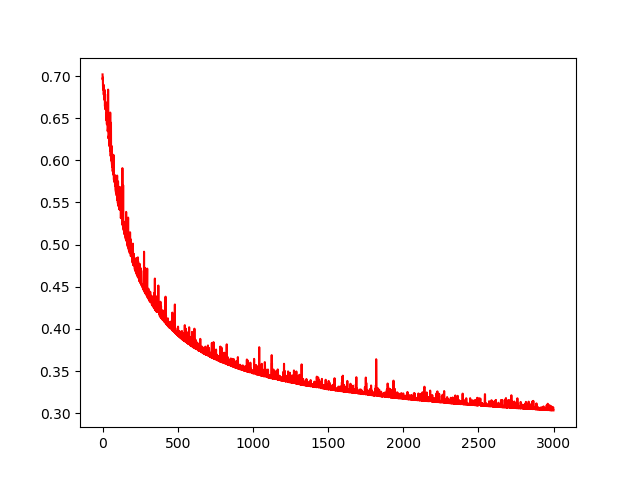
\includegraphics[width = .8\textwidth]{SGD100}
    \caption{p = 100}
    \label{SGD100}
\end{figure}

\subsection{BFGS}
\begin{table}[htbp]
    \caption{BFGS}
    \label{BFGS-table}
    \centering
    \begin{tabular}{lll}
      $\lambda$     &  1e-3 \\
      $\epsilon$     &  1e-5     \\
      step length     &   100 \\
      accuracy & 92.9\% 
    \end{tabular}
  \end{table}

\begin{figure}[htbp]
    \centering
    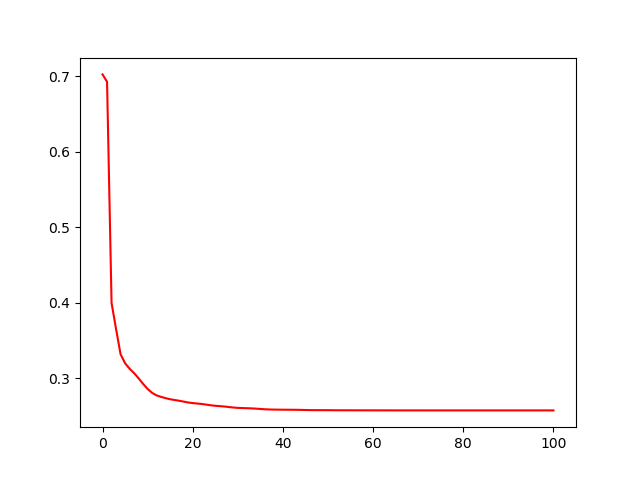
\includegraphics[width = .8\textwidth]{BFGS2}
    \caption{}
    \label{BFGS2}
\end{figure}

\subsection{LBFGS}
\begin{table}[htbp]
    \caption{LBFGS}
    \label{LBFGS-table}
    \centering
    \begin{tabular}{lll}
      $\lambda$     &  1e-3 \\
      $\epsilon$     &  1e-5     \\
      step length     &   50 \\
      accuracy & 90.7\% 
    \end{tabular}
  \end{table}

\begin{figure}[htbp]
    \centering
    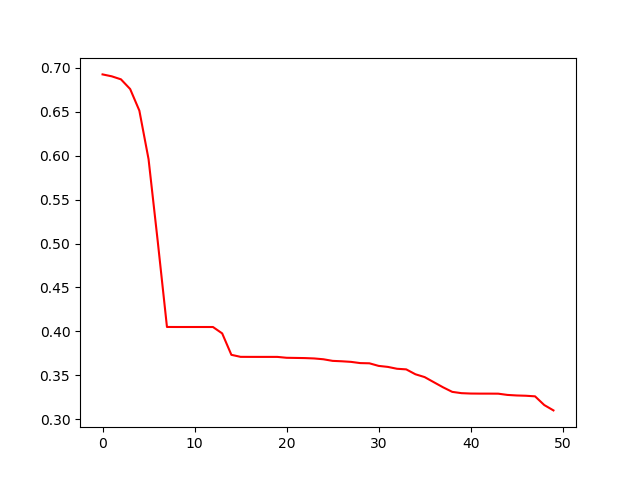
\includegraphics[width = .8\textwidth]{LBFGS}
    \caption{}
    \label{LBFGS}
\end{figure}

Remark that the convergence is not stable


\section{EM}
\subsection{E step:}
\begin{align}
Q_i(z_i) &= p(z_i \rvert x_i ; \theta)  \nonumber \\
& = \dfrac{p(z_i ,  x_i \rvert \theta)}{\sum_{z_i}p(z_i,  x_i \rvert \theta)} \nonumber \\
& = \dfrac{\pi_{z_i} \prod_{j = 1}^{M}\mu_{z_i}(j)^{x_i(j)}}{\sum_{z_i}^{k}\pi_{z_i} \prod_{j = 1}^{M} \mu_{z_i}(j)^{x_i(j)} }\nonumber 
\end{align}

\subsection{M step:}
\begin{align}
\mathcal{L}(\theta) & = \sum_{i = 1}^{N} \sum_{z_i} Q_i(z_i) \log \dfrac{p(x_i , z_i; \theta)}{Q_i(z_i)} \nonumber \\
& = \sum_{i = 1}^{N} \sum_{z_i} Q_i(z_i) \log p(x_i , z_i; \theta) - \sum_{i = 1}^{N} \sum_{z_i} Q_i(z_i) \log Q_i(z_i) \nonumber \\
& = Q(\theta) - const  \nonumber 
\end{align}
\begin{align}
\mathcal{Q}(\theta) & =  \sum_{i = 1}^{N} \sum_{z_i} Q_i(z_i) \log p(x_i , z_i; \theta)\nonumber \\
 & = \sum_{i = 1}^{N} \sum_{z_i}  \tau_{i,z_i} (\log \pi_{z_i} + \log  \prod_{j = 1}^{M}\mu_{z_i}(j)^{x_i(j)})\nonumber \\
 & = \sum_{i = 1}^{N} \sum_{z_i}  \tau_{i,z_i} (\log \pi_{z_i} + x_i(q)\log \mu_{z_i}(q)) \qquad (x_i(q) = 1)\nonumber 
\end{align}
Where we write $Q_i(z_i)$ as $\tau_{i,z_i}$.

There are 2 constraints: $\sum_{j}^{M}\mu_k(j) = 1$, $\sum_{i}^{K}\pi_i = 1$, with an observation $\sum_{j}^{M}x_i(j) = 1 \ \forall x_i \in \{ x_1, \ldots , x_N\}$. 

Use lagrange multiplier to find the optimum value of $\pi_{z_i}$ and $\mu_{z_i}$ as below:
\begin{align}
L(\mu, \pi, \lambda_1, \lambda_2) & = \mathcal{Q}(\pi, \mu) - \lambda_1 (\sum_{j}^{M}\mu_k(j) - 1) - \lambda_2 (\sum_{i}^{K}\pi_i  - 1) \nonumber \\
\dfrac{\partial L}{\partial \pi_k} &= \sum_{i = 1}^{N} \tau_{i,k} \frac{1}{\pi_k} - \lambda_2 = 0 \nonumber \\
sum\  \Rightarrow \ 1& = \sum_{k = 1}^{K} \pi_k = \frac{1}{\lambda_2} \sum_{k = 1}^{K}  \sum_{i = 1}^{N} \tau_{i,k}  \nonumber \\
\Rightarrow \lambda_2 &= \sum_{k = 1}^{K}  \sum_{i = 1}^{N} \tau_{i,k} \nonumber \\
plug\ in\Rightarrow \pi_k &= \dfrac{ \sum_{i = 1}^{N} \tau_{i,k}}{\sum_{k = 1}^{K}  \sum_{i = 1}^{N} \tau_{i,k}} \nonumber  \\
\qquad \nonumber \\
\dfrac{\partial L}{\partial \mu_k(q)} &=    \sum_{i = 1}^{N} \tau_{i,k} x_i(q) \frac{1}{\mu_k(q)} - \lambda_1 = 0 \nonumber \\
\Rightarrow \mu_k(q) &= \sum_{i = 1}^{N} \tau_{i,k} x_i(q) \frac{1}{\lambda_1} \nonumber \\
sum\ \Rightarrow \ 1&=\sum_{q=1}^{M}\mu_k(q) = \sum_{i = 1}^{N} \tau_{i,k} \sum_{q = 1}^{M}x_i(q) \frac{1}{\lambda_1} \nonumber \\
\Rightarrow \lambda_1 &= \sum_{i = 1}^{N}\tau_{i,k}   \nonumber \\
plug\ in \Rightarrow  \mu_k(q) &= \sum_{i = 1}^{N}\frac{ \tau_{i,k} x_i(q)}{\sum_{i = 1}^{N}\tau_{i,k}  } \nonumber
\end{align} 

To conclude, the probability for class $z = k$ is $ \pi_k = \dfrac{ \sum_{i = 1}^{N} \tau_{i,k}}{\sum_{k = 1}^{K}  \sum_{i = 1}^{N} \tau_{i,k}}$, the probability of $x_i$ which belongs to the class $z = k$ taking on the $q^{th}$ value is $\mu_k(q) = \dfrac{ \sum_{i = 1}^{N}\tau_{i,k} x_i(q)}{\sum_{i = 1}^{N}\tau_{i,k}  }$.

\section{VC-dimension}

\subsection{a}
The VC-dimension $h = 1$,

Justification: the case for 1 point is trivial, I can adjust the radius to label it as positive or negative no matter what the position is;
For case of 2 points, once the distance from the 2 points to the original point is different, then there's no way to classify them if the outer one is negative
and the inner one is positive as $\ref{prob31}$ shows.

\begin{figure}
    \centering
    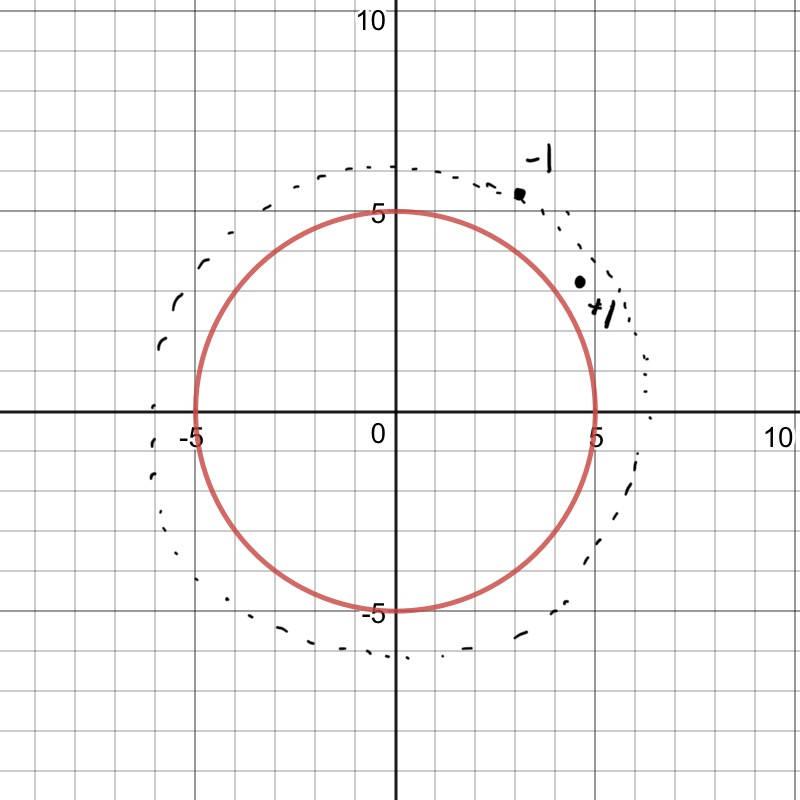
\includegraphics[width = .6\textwidth]{prob31}
    \caption{}
    \label{prob31}
\end{figure}



\subsection{b}
The VC-dimension $h = 2$,

Justification: Since I can reverse the classier by changing the sign of a, b, the case for 2 points is trivial as the inner one can be labeled as positive no matter how the
another is labeled; For the case of 3 points, as $\ref{prob32}$ illustrates, no matter where the third point is, its label will put some restriction on the labeling of
other points, for instance if the third point is in region (c) and be labeled negative, then either the intermedian point will be "sandwiched" and forced to be negative
or the inner one will be forced to be positive, and the situation is the same with region (a) and (b).

\begin{figure}
    \centering
    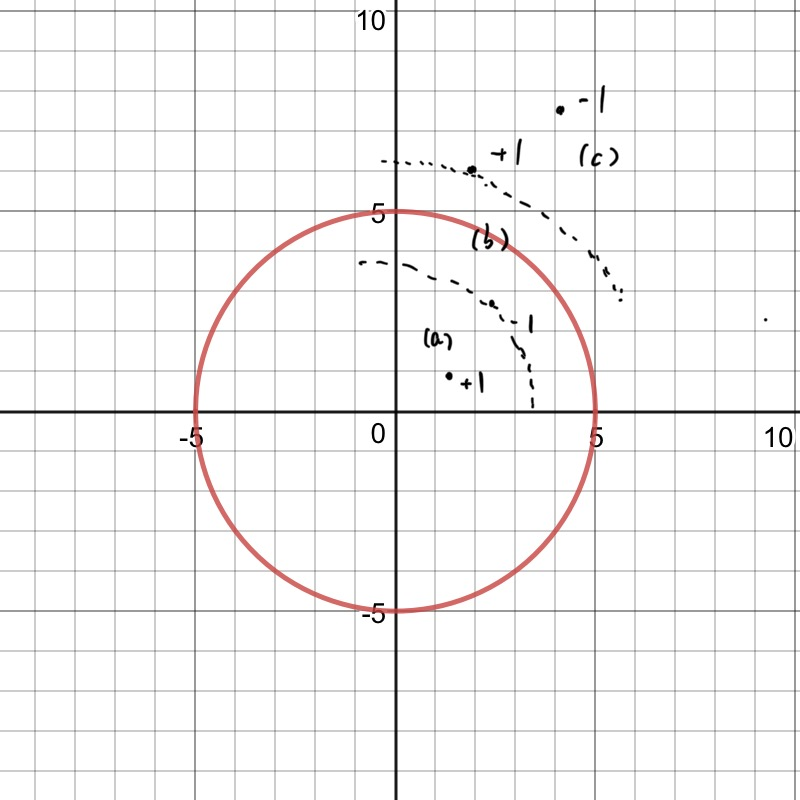
\includegraphics[width = .6\textwidth]{prob32}
    \caption{}
    \label{prob32}
\end{figure}



\end{document}